% !TEX program = pdflatex
% !BIB program = bibtex
% !TEX enableSynctex = true

\documentclass[12pt]{article}
\usepackage[utf8]{inputenc}
\usepackage{setspace}
\onehalfspacing
\usepackage{graphicx}
\usepackage{float}
\usepackage{appendix}
\renewcommand{\thesection}{\arabic{section}} 
\renewcommand{\thesubsection}{\thesection.\arabic{subsection}}
\usepackage{pdflscape}
\usepackage{color}   %May be necessary if you want to color links
\usepackage[colorlinks = true,
            linkcolor = blue,
            urlcolor  = blue,
            citecolor = blue,
            anchorcolor = blue]{hyperref}
\hypersetup{
    colorlinks=true, %set true if you want colored links
    linktoc=all,     %set to all if you want both sections and subsections linked
    linkcolor=blue,  %choose some color if you want links to stand out
}
\usepackage{algpseudocode}
\usepackage{algorithm}
\usepackage{bbm}

%For margins
\textheight = 22.62cm
\textwidth = 15.92cm
\topmargin = -0.54cm
\oddsidemargin= 0cm
\parindent=05mm
\usepackage{dashrule}
\usepackage{booktabs}
\usepackage{bbold}
\usepackage{amsmath}

\newtheorem{theorem}{Theorem}
\newtheorem{remark}{Remark}
\newtheorem{definition}[theorem]{Definition}
\DeclareMathOperator{\trace}{trace}
\DeclareMathOperator{\Var}{Var}

%Title Definition
\title{{\Large \vspace{-5em} \textbf{KSS Bias Correction : Outline} }}
\author{}
\date{}

\begin{document}
\maketitle

\section{Introduction}
Consider a linear model with nonrandom $x_i \in \mathbbm{R}^k$. 

\begin{align*}
    y_i = x_i' \beta + \varepsilon_i
\end{align*}
where $i = 1,\dots,n$ and $\varepsilon \sim N(0, \sigma_i^2)$.

\begin{definition}
A (co)variance component is a quadratic form $\theta = \beta' A \beta $, where $A$ is a $k\times k$ matrix. When A is positive semi-definite we call it a variance component and when A is non-definite we call it covariance component.
\end{definition}

\begin{remark}
The plug-in estimator for the (co)variance component $\theta$ is biased. In particular, we can write 

\begin{align*}
    \mathbbm{E}(\hat{\theta}) = \theta + \underbrace{ \trace(A \Var(\hat{\beta}))}_\text{bias}
\end{align*}

\noindent And the bias term can be written as $\sum_{i=1}^n B_{ii} \sigma_i^2$, where $B_{ii} = x_i' S_{xx}^{-1} A S_{xx}^{-1} x_i  $, $S_{xx} = \sum_{i=1}^n x_i x_i'$.
\end{remark}

\begin{remark}
The previous remark suggest that we can estimate the bias as

\begin{align*}
    \hat{bias} &= \sum_{i=1}^n B_{ii} \hat{\sigma_i}^2 \\    
    \hat{\sigma_i}^2 &= y_i (y_i - x_i' \hat{\beta}_{-i}) = y_i \frac{(y_i - x_i ' \hat{\beta})}{1-P_{ii}}\\
\end{align*}
where $P_{ii}$ is the statistical leverage of observation $i$, and it's defined as $P_{ii} := (X (X'X) X')_{ii}$.

\end{remark}

\clearpage
\begin{remark}
If we compute $\hat{\beta}$, $B_{ii}$ and $P_{ii}$ then we can compute the ``bias-corrected'' estimator of the (co)variance components

\begin{align*}
    \hat{\theta}_{KSS} =  \hat{\beta}' A \hat{\beta} - \sum_{i=1}^n B_{ii} y_i \frac{(y_i - x_i ' \hat{\beta})}{1-P_{ii}}
\end{align*}
\end{remark}

\vspace{0.5cm}
Our model of interest is the two-way fixed effects model given by

\begin{align*}
y_{gt} = \alpha_{g} + \psi_{j(g,t} + x_{gt}' \delta + \varepsilon_{gt}
\end{align*}


\noindent where $g \in \{1,\dots,N\}$ denotes the worker identity, $t$ denotes the time period, $j(g,t) \in \{1,\dots,J\}$ denotes the firm of worker $g$ at time $t$. Moreover, we can index the observations using $i$ instead of $g,t$ and we will denote $n$ as the total number of observations. 

The (co)variance components in this context take the form 

\begin{align*}
    \sigma_{\psi}^2 &= \frac{1}{n} \sum_{g=1}^{N} \sum_{t=1}^{T_g} (\psi_{j(g,t)} - \Bar{\psi})^2  \\
    \sigma_{\alpha, \psi}^2 &= \frac{1}{n} \sum_{g=1}^{N} \sum_{t=1}^{T_g} (\psi_{j(g,t)} - \Bar{\psi}) \alpha_g  \\
    \sigma_{\alpha}^2 &= \frac{1}{n} \sum_{g=1}^{N} \sum_{t=1}^{T_g} (\alpha_{g} - \Bar{\alpha})^2   \\
\end{align*}
where $\Bar{\psi} = \frac{1}{n} \sum_{g=1}^{N} \sum_{t=1}^{T_g} \psi_{j(g,t)}$. Let $f_i = (\boldsymbol{1}_{\{j(g,t)=1\}},\dots,\boldsymbol{1}_{\{j(g,t)=J\}})'$ and $d_i = (\boldsymbol{1}_{\{g=1\}},\dots,\boldsymbol{1}_{\{g=N\}})'$ . We can compute the (co)variance components in this model in quadratic forms using the following $A$ matrices

\begin{align*}
A_{\psi} = \begin{bmatrix}
0 & 0 & 0\\
0 & A_{ff} & 0\\
0 & 0 & 0
\end{bmatrix} \quad \text{where} \quad A_{ff} = \frac{1}{n} \sum_{i=1}^n (f_i - \Bar{f})(f_i - \Bar{f})'
\end{align*}

\begin{align*}
A_{\alpha,\psi} = \begin{bmatrix}
0 & A_{df} & 0\\
A_{df}' & 0 & 0\\
0 & 0 & 0
\end{bmatrix} \quad \text{where} \quad A_{df} = \frac{1}{n} \sum_{i=1}^n (d_i - \Bar{d})(f_i - \Bar{f})'
\end{align*}

\begin{align*}
A_{\alpha} = \begin{bmatrix}
A_{dd} & 0 & 0\\
0 & 0 & 0\\
0 & 0 & 0
\end{bmatrix} \quad \text{where} \quad A_{dd} = \frac{1}{n} \sum_{i=1}^n (d_i - \Bar{d})(d_i - \Bar{d})'
\end{align*}



\section{Matrix Form of the Model}

Define the dummy variable matrices

\begin{align*}
    \underbrace{D}_\text{Worker Dummies} &= \underbrace{\begin{bmatrix} \boldsymbol{1}_{\{g=1\}} \iota_n \dots \boldsymbol{1}_{\{g=N\}} \iota_n  \end{bmatrix}}_\text{One non-zero value per row at most} \quad \text{where} \quad \iota_n = (1, \dots, 1)' \in \mathbbm{R}^n
\end{align*}

\begin{align*}
    \underbrace{F*S}_\text{Firm Dummies} &= \underbrace{\begin{bmatrix} \boldsymbol{1}_{\{j(g,t)=1\}} \iota_n \dots \boldsymbol{1}_{\{j(g,t)=J\}} \iota_n  \end{bmatrix}}_\text{One non-zero value per row at most} * \underbrace{\begin{bmatrix} I_{J-1} & 0 \\ 0 & 0 \end{bmatrix}}_\text{Normalize last firm effect to 0}
    \quad \text{where} \quad I_{J-1}:= \text{identity matrix}
\end{align*}


\begin{align*}
    \underbrace{C}_\text{Control Variables} &= \begin{bmatrix} x_1' \\ \vdots \\ x_n'  \end{bmatrix}
\end{align*}

Then we can write the model in matrix form as

 \begin{align*}
     Y &= \begin{bmatrix} D & F*S & C \end{bmatrix} \begin{bmatrix} \alpha \\ \psi \\ \delta \end{bmatrix} + \varepsilon\\
     &= X \beta + + \varepsilon
\end{align*}
          
And we can estimate $\beta$ by solving the least-squares problem, and notice that the design matrix, $X$, is very sparse based on the definitions of $D$ and $F*S$.



\section{Computation of $B_{ii}$ and $P_{ii}$}

It can be shown that 

\begin{align*}
    P_{ii} = x_i' S_{xx}^{-1} x_i \quad \text{and} \quad B_{ii} = x_i' S_{xx}^{-1} A  S_{xx}^{-1} x_i
\end{align*}

\noindent But in practice the computation of $S_{xx}^{-1}$ can be difficult given the high dimension of parameters in the model. The approach taken in KSS is to avoid the computation of this inverse and instead compute 

\begin{align*}
    z_i^{exact} = S_{xx}^{-1} x_i \quad \text{for each} \quad i=1,\dots,n
\end{align*}

In other words, we solve separately for each column of $Z$ in the following system

\begin{align*}
    \underbrace{S_{xx}}_{k\times k} \underbrace{Z_{exact}}_{k\times n}  = \underbrace{X'}_{k\times n}
\end{align*}

\noindent With that solution we compute $P_{ii} = x_i' z_i^{exact}$ and $B_{ii} = {z_i^{exact}}' A z_i^{exact}$


\begin{remark}
Exact computation can be infeasible given the dimensionality of the problem. The authors propose a dimension reduction via Rademacher matrices, also known as Johnson-Lindenstrauss Approximation (JLA). In particular, it consists on transforming the system so that we only require to solve $p$ systems instead of $n$ systems, where $p$ can be significantly smaller than $n$.

In other words, we solve separately for each column of Z in the following system

\begin{align*}
    \underbrace{S_{xx}}_{k\times k} \underbrace{Z_{JLA}}_{k\times p}  = \underbrace{(R_p *X)'}_{k\times p}
\end{align*}


\end{remark}

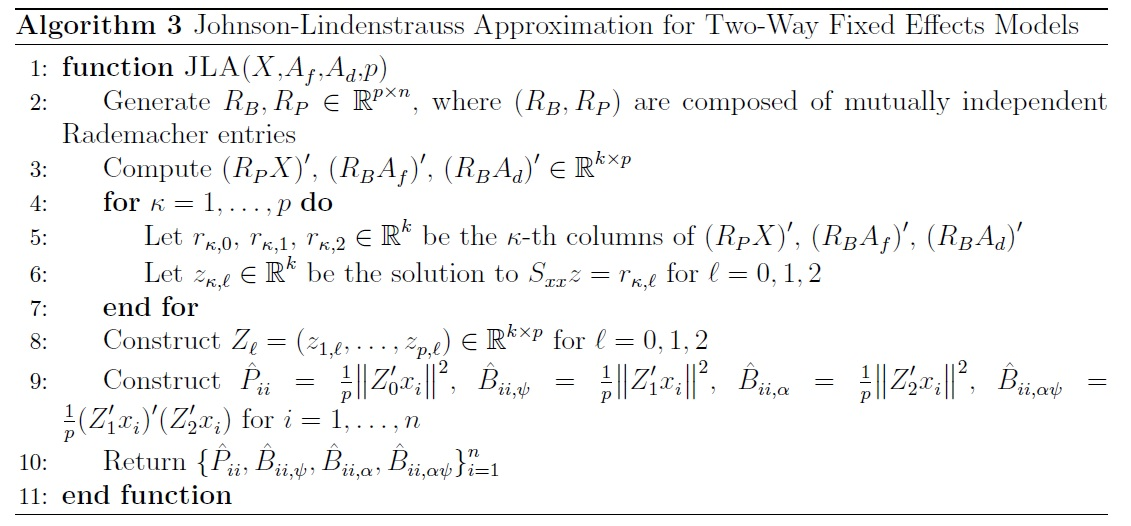
\includegraphics[scale=0.7]{JLA_algorithm.jpg}

\begin{remark}
When there are no controls in the design matrix, the model simplifies to
\begin{align*}
    X = \begin{bmatrix} D & F*S \end{bmatrix} \quad \beta = \begin{bmatrix} \alpha \\ \psi \end{bmatrix} 
\end{align*}

\noindent Moreover, there's no loss of generality of rewriting as
\begin{align*}
    X = \begin{bmatrix} D & -F*S \end{bmatrix} \quad \beta = \begin{bmatrix} \alpha \\ -\psi \end{bmatrix} 
\end{align*}

\noindent If we do this $X'X$ is symmetric and diagonally dominant, and the normal equations can be solved as a Laplacian system. This is where the preconditioner \textit{CMG} comes into play in the code.


\end{remark}


\section{Leave-One-Out for Clusters}

We can extend this framework to allow for leave-out estimation of clusters of observations. Suppose there are $c\in \{1,C\}$ clusters of $n_c$ observations. We can redefine the model as follows

\begin{align*}
    y_c = X_c \quad \beta + \varepsilon_c 
\end{align*}

\begin{align*}
    y_c = \begin{bmatrix} y_{c,1} \\ \vdots \\ y_{c,n_c}  \end{bmatrix} \quad X_c = \begin{bmatrix} x_{c,1}' \\ \vdots \\ x_{c,n_c}'  \end{bmatrix} \quad \varepsilon_c = \begin{bmatrix} \varepsilon_{c,1} \\ \vdots \\ \varepsilon_{c,n_c}  \end{bmatrix} 
\end{align*}

In this case, we can define an analogue for the bias corrected estimator

\begin{align*}
    \hat{\theta}_{KSS} =  \hat{\beta}' A \hat{\beta} - \sum_{i=c}^C y_c' B_c (1- P_c)^{-1} (y_c - X_c   \hat{\beta})
\end{align*}

where

\begin{align*}
    P_c = X_c S_{xx}^{-1} X_c' = \underbrace{ \begin{bmatrix} x_{c,1}' S_{xx}^{-1}  x_{c,1} & \dots & x_{c,1}' S_{xx}^{-1}  x_{c,n_c}  \\ \vdots & \vdots & \vdots \\ x_{c,n_c}' S_{xx}^{-1}  x_{c,1} & \dots & x_{c,1}' S_{xx}^{-1}  x_{n_c,n_c} \end{bmatrix} }_\text{From symmetry we only need to compute upper or lower triangular half }
\end{align*}

\begin{align*}
    B_c = X_c S_{xx}^{-1} A S_{xx}^{-1} X_c' = \underbrace{ \begin{bmatrix} x_{c,1}' S_{xx}^{-1} A S_{xx}^{-1} x_{c,1} & \dots & x_{c,1}' S_{xx}^{-1} A S_{xx}^{-1} x_{c,n_c}  \\ \vdots & \vdots & \vdots \\ x_{c,n_c}' S_{xx}^{-1} A S_{xx}^{-1}  x_{c,1} & \dots & x_{c,1}' S_{xx}^{-1} A S_{xx}^{-1}  x_{n_c,n_c} \end{bmatrix} }_\text{From symmetry we only need to compute upper or lower triangular half }
\end{align*}

Now, we can solve $M$ systems of equations and solve for
 \begin{align*}
     z_{c,l}^{exact} = S_{xx}^{-1} x_{c,l} \quad \text{where} \quad c\in\{1,\dots,C\} \quad and \quad l\in\{1,\dots,n_c\}
 \end{align*}

The function \textit{index\_constr()} is the one in charge of computing which observations belong to the same cluster, so that we only need to compute $M$ numbers because of the symmetry of these matrices.


\clearpage
\appendix

\section{Simple Network Example}

Suppose we are given the following dataset

\begin{table}[h!]
    \centering
\begin{tabular}{|c c c c|} 
 \hline
 id & year & firmid & outcome \\ [0.5ex] 
 \hline\hline
 1 & 1 & A &  0,1462\\ 
 \hline
 1 & 2 & B & 0,2968 \\
 \hline
 2 & 1 & A &  0,5434\\
 \hline
 2 & 2 & A & 0,4326 \\
 \hline
 3 & 1 & A & 0,4648 \\
 \hline
 4 & 1 & A & 0,7306 \\
 \hline
 4 & 2 & B & 0,6192 \\
 \hline
 5 & 1 & B &  0,7534\\
 \hline
 5 & 2 & B &  0,0863\\
 \hline
6 & 1 & B &  0,3720\\
 \hline
 6 & 2 & C & 0,9580 \\ [1ex] 
 \hline
\end{tabular}
\end{table}

We can write the corresponding bipartite graph as follows
\begin{figure}[h!]
    \centering
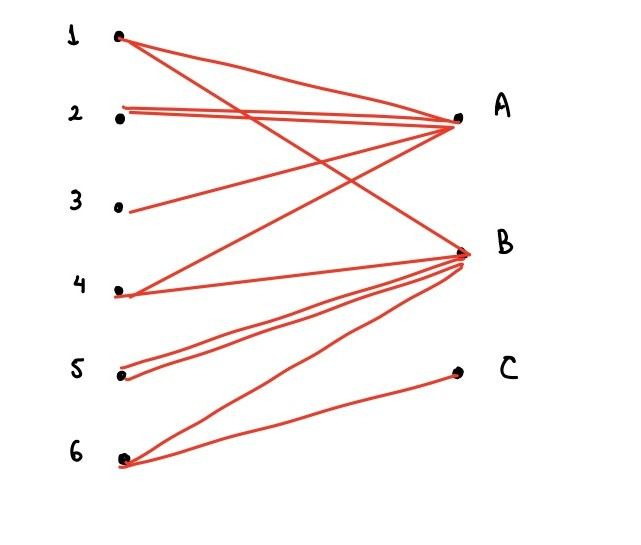
\includegraphics[scale=0.7]{minimal_unit.png}    \end{figure}

The function $\textit{find\_connected\_set()}$ will find the largest connected component of this network, which corresponds to the whole network. This means that we can estimate the coefficients for every worker effect and every firm effect. 

Now, the function $\textit{prunning\_connected\_set()}$ will prune the worker vertex that are articulation points and find the largest connected set until no more articulation points are found. In this network it corresponds to worker 6, so all of its edges will be pruned. Notice that this will disconnect firm C with the rest of the network. After that, the network is also the largest connected component with no more articulation points, so the function stops at that point. The network that we get as an output is the following

\begin{figure}[h!]
    \centering
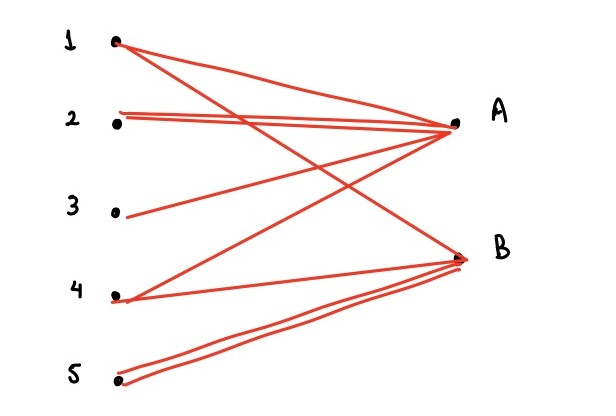
\includegraphics[scale=0.7]{pruning.png}    
\end{figure}

Finally, the function $\textit{drop\_single\_obs()}$ will delete the workers that only have one observation(edge). In this particular case it corresponds to worker 3. We are required to prune these workers because once we leave-out that observation we can no longer estimate the coefficient for worker 3's effect. Therefore, the leave-one-out connected set is structured as follows

\begin{figure}[h!]
    \centering
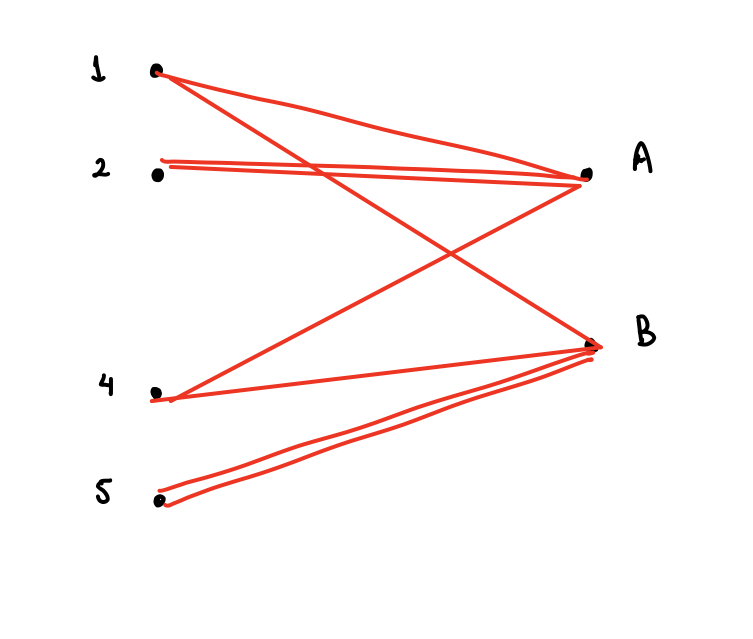
\includegraphics[scale=0.6]{leaveoutnetwork.png}    
\end{figure}





\end{document}
